\documentclass{article}
\usepackage{amsmath}
\usepackage{enumerate}
\usepackage{fancyhdr} % Required for custom headers
\usepackage{lastpage} % Required to determine the last page for the footer
\usepackage{extramarks} % Required for headers and footers
\usepackage[usenames,dvipsnames]{color} % Required for custom colors
\usepackage{graphicx} % Required to insert images
\usepackage[tight,footnotesize]{subfigure} % Required for subfig
\usepackage{caption} % Required for subfig
\usepackage{hyperref} % Required for url
\usepackage{listings} % Required for insertion of code
\usepackage{courier} % Required for the courier font
\usepackage{lipsum} % Used for inserting dummy 'Lorem ipsum' text into the template
\topmargin=-0.45in
\evensidemargin=0in
\oddsidemargin=0in
\textwidth=6.5in
\textheight=9.0in
\headsep=0.25in
\linespread{1.1} % Line spacing
\pagestyle{fancy}
\lhead{\hmwkAuthorName} % Top left header
% \chead{\hmwkClass\ (\hmwkClassInstructor\ \hmwkClassTime): \hmwkTitle} % Top center head
\chead{\hmwkClass\ : \hmwkTitle} % Top center head
\rhead{\firstxmark} % Top right header
\lfoot{\lastxmark} % Bottom left footer
\cfoot{} % Bottom center footer
\rfoot{Page\ \thepage\ of\ \protect\pageref{LastPage}} % Bottom right footer
\renewcommand\headrulewidth{0.4pt} % Size of the header rule
\renewcommand\footrulewidth{0.4pt} % Size of the footer rule
\setlength\parindent{0pt} % Removes all indentation from paragraphs

% Define floor and ceiling
\def\lc{\left\lceil}   
\def\rc{\right\rceil}
\def\lf{\left\lfloor}   
\def\rf{\right\rfloor}

% Set your language 
%\lstset{language=Java}
\definecolor{codegreen}{rgb}{0,0.6,0}
\definecolor{codegray}{rgb}{0.5,0.5,0.5}
\definecolor{codepurple}{rgb}{0.58,0,0.82}
\definecolor{backcolour}{rgb}{0.95,0.95,0.92}
 
\lstdefinestyle{mystyle}{
    backgroundcolor=\color{backcolour},   
    commentstyle=\color{codegreen},
    keywordstyle=\color{magenta},
    numberstyle=\tiny\color{codegray},
    stringstyle=\color{codepurple},
    basicstyle=\footnotesize,
    breakatwhitespace=false,         
    breaklines=true,                 
    captionpos=b,                    
    keepspaces=true,                 
    numbers=left,                    
    numbersep=8pt,                  
    showspaces=false,                
    showstringspaces=false,
    showtabs=false,                  
    tabsize=2
}
\lstset{style=mystyle}

% Header and footer for when a page split occurs within a problem environment
\newcommand{\enterProblemHeader}[1]{
\nobreak\extramarks{#1}{#1 continued on next page\ldots}\nobreak
\nobreak\extramarks{#1 (continued)}{#1 continued on next page\ldots}\nobreak
}

% Header and footer for when a page split occurs between problem environments
\newcommand{\exitProblemHeader}[1]{
\nobreak\extramarks{#1 (continued)}{#1 continued on next page\ldots}\nobreak
\nobreak\extramarks{#1}{}\nobreak
}

\setcounter{secnumdepth}{0} % Removes default section numbers
\newcounter{homeworkProblemCounter} % Creates a counter to keep track of the number of problems

\newcommand{\homeworkProblemName}{}
\newenvironment{homeworkProblem}[1][Problem \arabic{homeworkProblemCounter}]{ % Makes a new environment called homeworkProblem which takes 1 argument (custom name) but the default is "Problem #"
\stepcounter{homeworkProblemCounter} % Increase counter for number of problems
\renewcommand{\homeworkProblemName}{#1} % Assign \homeworkProblemName the name of the problem
\section{\homeworkProblemName} % Make a section in the document with the custom problem count
\enterProblemHeader{\homeworkProblemName} % Header and footer within the environment
}{
\exitProblemHeader{\homeworkProblemName} % Header and footer after the environment
}

\newcommand{\problemAnswer}[1]{ % Defines the problem answer command with the content as the only argument
\noindent\framebox[\columnwidth][c]{\begin{minipage}{0.98\columnwidth}#1\end{minipage}} % Makes the box around the problem answer and puts the content inside
}

\newcommand{\homeworkSectionName}{}
\newenvironment{homeworkSection}[1]{ % New environment for sections within homework problems, takes 1 argument - the name of the section
\renewcommand{\homeworkSectionName}{#1} % Assign \homeworkSectionName to the name of the section from the environment argument
\subsection{\homeworkSectionName} % Make a subsection with the custom name of the subsection
\enterProblemHeader{\homeworkProblemName\ [\homeworkSectionName]} % Header and footer within the environment
}{
\enterProblemHeader{\homeworkProblemName} % Header and footer after the environment
}

\newlength{\tabcont}

\newcommand{\tab}[1]{%
\settowidth{\tabcont}{#1}%
\ifthenelse{\lengthtest{\tabcont < .25\linewidth}}%
{\makebox[.25\linewidth][l]{#1}\ignorespaces}%
{\makebox[.5\linewidth][l]{\color{red} #1}\ignorespaces}%
}%
%----------------------------------------------------------------------------------------------
%	NAME AND CLASS SECTION
%----------------------------------------------------------------------------------------------

\newcommand{\hmwkTitle}{Homework\ \#8} % Assignment title
\newcommand{\hmwkDueDate}{Monday,\ January\ 1,\ 2012} % Due date
\newcommand{\hmwkClass}{Fundamental Algorithms} % Course/class
\newcommand{\hmwkClassTime}{} % Class/lecture time
\newcommand{\hmwkClassInstructor}{Prof. Joel Spencer} % Teacher/lecturer
\newcommand{\hmwkAuthorName}{Songxiao Zhang, N10224459, {\tt 72}} % Your name

%----------------------------------------------------------------------------------------------
%	TITLE PAGE
%----------------------------------------------------------------------------------------------

\title{
\textmd{\textbf{\hmwkClass:\ \hmwkTitle}}\\
}
\author{\textbf{\hmwkAuthorName}}

\begin{document}

\maketitle

%----------------------------------------------------------------------------------------------
%	PROBLEM 1
%----------------------------------------------------------------------------------------------
\begin{homeworkProblem}

According to the property of Huffman code, $$A[i].right = A[i].left.right + A[i].left.left$$ for any node $i$ in a tree keeps growing to the left side. (Similar for a tree growing right, $$A[i].left = A[i].right.left + A[i].right.right)$$ So in level-1 ($i$ is the root), the code word length is 1, $0$ or $1$, $z$ must have the largest frequency in a left-growing tree among
$$(z, z.parent.left.left, z.parent.left.right)$$
so that $z$ is in level-1 with code length 1, $z.parent.left.left$ and $z.parent.left.right$ are in level-2 with code length 2. Similar reason in a right-growing tree, $z$ needs to have the maximum frequency among the 3 nodes of $(z, z.parent.right.left, z.parent.right.right)$.
Then $z.frequency \geq \frac{1}{3}$ is true. \\

An example of $z.frequency = 0.36$ in a left growing tree is given in Figure~\ref{fig:forz} on Page~\pageref{fig:forz}.
\begin{figure}[h!]
    \centering
    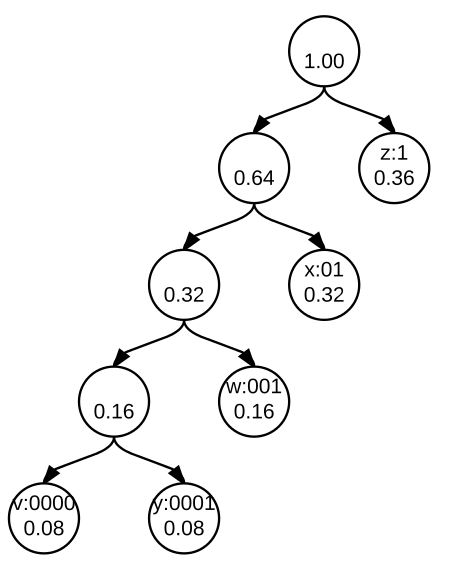
\includegraphics[scale=0.4]{hw8/2.png}
    \caption{}
    \label{fig:forz}
\end{figure} 
% According to the property of Huffman code $f_a >= f_b + f_c$ where $a$ is the sibling of the 
% parent of $b$ and $c$, assume the frequency of code words at the same level are the same, 
% we can build a equation that for a dictionary with 5 words
% $$ \sum\limits_{i=1}^{5} f_i + f_5 = 1, f_i \geq 2 * f_{i-1}$$
% where $f_i$ stands for frequency of level $i$ code word with length $i$. 
% $\sum\limits_{i=1}^{5} \frac{1}{2^{i-1}} * f_1 \geq 1$ so $f_1 \geq 0.5$. 
% Since the frequency of the right child can be larger than the left one (we assumed them equal
% at first), $f_1$ can get smaller than this value. 
% Thus, for code book $\{v,w,x,y,z\}$, if $z$ is 0 or 1 at level 1, 
% its frequency cannot be less than $\frac{1}{3}$. \\

% If $f_z = 0.36$ where $z$ is 0 or 1, the total frequency of the code book is 
% $$TotalFrequency \geq 0.36 * 2 + 0.36 / 2 * 3 = 1.26$$ which is larger than 1 and it's
% impossible. 
% The example can be \\
% $z$(0, 0.36), $y$(0, 0.36)
% ROOT.LEFT = $z$(0, 0.36), ROOT.RIGHT = $y$(1, 0.36), \\
% $z$.LEFT = $x$(0, 0.18), $z$.RIGHT = $w$(1, 0.18), $y$.RIGHT = $x$(0, 0.18)\\
% If the frequency of some right child is smaller than the one of the left, the sum of frequency 
% can get even smaller. 
\end{homeworkProblem}

%----------------------------------------------------------------------------------------------
%	PROBLEM 2
%----------------------------------------------------------------------------------------------
\begin{homeworkProblem}
The algorithm traverse the activities from the latest starting time. If finished before
the last started, then current one is added to the optimal solution. The first activity with 
the latest starting time is chosen before other ones because the list of activities is sorted
in increasing order. 
\begin{lstlisting}[frame=single]
Selector(A)
    n = A.length
    sort A by A.s
    B is a list with size n
    tmps = A[n].s
    
    for i = n - 1 to 1
        if A[i].f <= tmps
            add A[i] to B
            tmps = A[i].s
    
    return B
\end{lstlisting}
$A$ is the input of an array of activities, each with start time $A[i].s$ and 
finish time $A[i].f$ for $i^{th}$ activity. 

$Proof: $ Sort $A$ with size n by the start time $A[i].f$ and $B$ is a maximum subset of 
mutually compatible activities of $A$. Let's denote $A[j].s = tmps$ in the code. 

If $A[i] == A[j]$, $A[i]$ is in a max-subset of mutually compatible activities sorted by
starting time. We’re done here. \\
If $A[i] != A[j]$, $B[k + 1] = B[k] - A[j] + A[i]$. $A[i]$ and $A[j]$ are both the latest
starting time so $A[i] = A[j]$ and so $B[k + 1] = B[k]$ is also a max-subset, and $A[j]$ is
in a max-subset of mutually compatible activities sorted by starting time.

\end{homeworkProblem}

%----------------------------------------------------------------------------------------------
%	PROBLEM 3
%----------------------------------------------------------------------------------------------
\begin{homeworkProblem}

\begin{enumerate}[(a)]
    \item $A: [[1, 5], [4, 7], [6, 10]]$ solution $[[4.7]]$ while optimal solution 
          $[[1, 5], [6, 10]]$   
    \item $A: [[0, 4], [4, 6], [6, 10], [0, 1], [1, 5], [5, 9], [9, 10], [0, 3], 
          [0, 2], [7, 10], [8, 10]]$ solution $[[4.6]]$ while optimal solution $
          [[0, 1], [1, 5], [5, 9], [9, 10]]$    
    \item $A: [[0, 10], [4, 6], [6, 10]]$ solution $[[0.10]]$ while optimal solution
          $[[4, 6], [6, 10]]$
\end{enumerate}

\end{homeworkProblem}

%----------------------------------------------------------------------------------------------
%	PROBLEM 4
%----------------------------------------------------------------------------------------------
\begin{homeworkProblem}
To add up the list {a: 1, b: 1, c: 2, d: 3, e: 5, f: 8, g: 13, h: 21} \\
The result is {1, 2, 4, 7, 12, 20, 33, 54}, and we can put 0 on the left and 1 on the right side.
Figure~\ref{fig:tree} on Page~\pageref{fig:tree}.
\begin{figure}[h!]
    \centering
    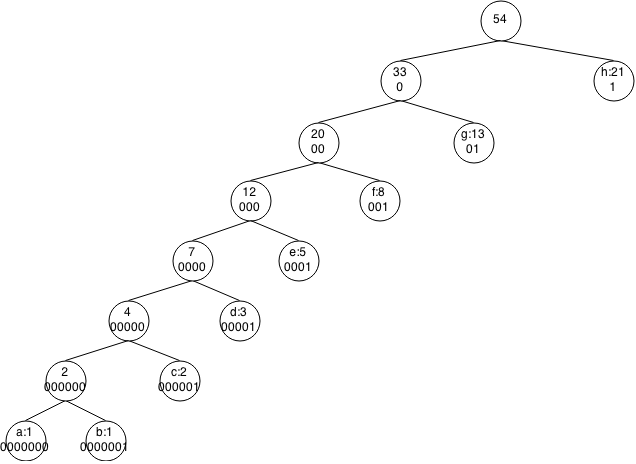
\includegraphics[scale=0.6]{hw8/1.png}
    \caption{Hard to draw 0 on the left branch and 1 on the right branch, so I put the code word in the node directly. }
    \label{fig:tree}
\end{figure} 

We can generalize the first $n$ (excluding the 0) Fibronacci numbers. $nth$ element is 1 and
the $(n-k)$

\begin{lstlisting}[frame=single]
function getithElementofNFib(n, k)
    for i from 1 to (n-k)
        append 0 to code
    if k != 0
        append 1 to code
    return code 
\end{lstlisting}

\begin{lstlisting}[frame=single]
# use python to print out the table
def getithElementofNFib(n, k):
    code = []
    for i in range(n - k - 1):
        code.append(0)

    if k != 0:
        code.append(1)
    return code

for i in range(8):
    print i, " ", getithElementofNFib(8, i)
\end{lstlisting}
   
% # use python to print out the table
% def getithElementofNFib(n, k):
%     code = []
%     for i in range(n - k - 1):
%             code.append(0)

%     if k != 0:
%         code.append(1)
%     return code

% for i in range(8):
%     print i, " ", getithElementofNFib(8, i)

A sample output for $n = 8$
\begin{lstlisting}[frame=single]
0   [0, 0, 0, 0, 0, 0, 0]
1   [0, 0, 0, 0, 0, 0, 1]
2   [0, 0, 0, 0, 0, 1]
3   [0, 0, 0, 0, 1]
4   [0, 0, 0, 1]
5   [0, 0, 1]
6   [0, 1]
7   [1]
\end{lstlisting}

\end{homeworkProblem}

%----------------------------------------------------------------------------------------------
%	PROBLEM 5
%----------------------------------------------------------------------------------------------
\begin{homeworkProblem}
Without using Min-heap, the data is stored in a linked list which looks like a flattened
binary tree, by storing the data of every node with $depth > 0$ in the the node of the 
linked list. We can take Problem 4 as an example. Instead of building a heap, we put them in a list
$$[a:[0, 1, 0000000],\ b:[2, 1, 0000001],\ c:[4, 2, 000001],\ d:[7, 3, 00001],\ 
e:[12, 5, 0001],..., h:[54, 21, 1]]$$
Traversing from root, the value of the next node is by inserting 0 at the head.\\

The running time is changed in the EXTRACTMIN(), which is now $\Theta(n)$ 
instead of $\Theta(\lg(n))$. Adding an element to list still $\Theta(1)$. The total running time now is $\Theta(n^2)$. 
\end{homeworkProblem}



% \begin{lstlisting}[frame=single]
% \end{lstlisting}

% \begin{enumerate}[a.]
%     \item 
        %   
        %   
% \end{enumerate}

% Figure~\ref{fig:tree} on Page~\pageref{fig:tree}.
% \begin{figure}[h!]
%     \centering
%     \subfigure[]{\label{}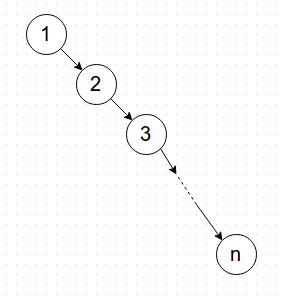
\includegraphics[scale=0.4]{hw6/51.png}}
%     \subfigure[]{\label{}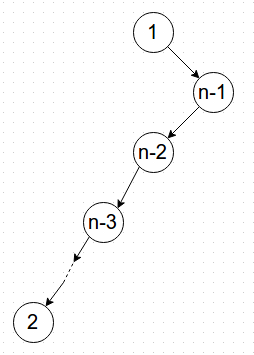
\includegraphics[scale=0.4]{hw6/52.png}}
%     \caption{}
%     \label{fig:tree}
% \end{figure} 
\end{document}